
% TODO: lacks a simple introduction to Generics
\documentclass[English,c,% 't' (resp. 'c') places text vertically at top/center of each slide
% PDF settings
hyperref={%
    pdftitle={FISA-DE2 OOP in Java},%
    pdfauthor={Muller, Gravier, Laforest, Subercaze},%
    pdfsubject={OOP in Java},%
    pdfkeywords={OOP, Java},%
    colorlinks=true,%
    urlcolor=blue,%
    linkcolor=%
    },%
% To load many pre-defined color names
xcolor={pdftex,svgnames} % dvipsnames, dvipsnames*, svgnames, svgnames*, x11names,
]{beamer}

\usetheme{Copenhagen}
%\setbeamertemplate{footline}[page number]
%\setbeamertemplate{frametitle}[default][center]
% To remove the navigation symbols from the bottom of slides:

% Remove navigation bar
\setbeamertemplate{navigation symbols}{}
% Remove outline at top
\setbeamertemplate{headline}{}

\addtobeamertemplate{navigation symbols}{}{%
    \usebeamerfont{footline}%
    \usebeamercolor[fg]{footline}%
    \hspace{1em}%
    \insertframenumber/\inserttotalframenumber
}

% Put text more on top of each slide for all slides
\addtobeamertemplate{frametitle}{}{\vspace*{-.7em}}

% Correct French/English indentation and splitting of words
\usepackage{babel}

% Correct management of accentuated chars in input file
\usepackage[utf8]{inputenc}

% Correct font for the generation of docs with accentuated chars
\usepackage[T1]{fontenc}      % Can handle hyphenation of words with accented characters
%%\usepackage[OT1]{fontenc}   % Might generated bad looking PDFs

% Insertion of images generated by external tools
\usepackage{graphicx}
% To generate pretty & scalable images directly in LaTeX
\usepackage{tikz}

% To print numbers correctly
\usepackage{numprint}

\usepackage[absolute,overlay]{textpos}

\usepackage{fourier}

\setbeamercovered{transparent}
\setbeamercovered{invisible}

\AtBeginSection[]
{
   \begin{frame}{Outline}
       \tableofcontents[currentsection]
   \end{frame}
}

\usepackage{url,manfnt}


% To be able to insert code listing
\usepackage{listings}

\definecolor{dkgreen}{rgb}{0,0.6,0}
\definecolor{gray}{rgb}{0.5,0.5,0.5}
\definecolor{mauve}{rgb}{0.58,0,0.82}

\lstset{frame=none,
  language=Java,
  aboveskip=1mm,
  belowskip=1mm,
  showstringspaces=false,
  columns=flexible,
  basicstyle={\scriptsize \ttfamily},
  numbers=left,
  numberstyle=\scriptsize\color{gray},
  keywordstyle=\color{blue},
  commentstyle=\color{dkgreen},
  stringstyle=\color{mauve},
  breaklines=true,
  breakatwhitespace=true,
  tabsize=2
}
\definecolor{algoTitle}{rgb}{0.84,0.83,0.94}

\usepackage{caption}
\DeclareCaptionFont{white}{\color{white}}
\DeclareCaptionFormat{listing}{\colorbox{algoTitle}{\parbox{\textwidth}{\bfseries #1#2 #3}}}
\captionsetup[lstlisting]{format=listing,labelfont=white,textfont=white}

\title[OOP in Java]{Object-Oriented Programming in \raisebox{-.3\height}{
\includegraphics[height=1.5em]{./images01/java_logo.png}}}
\logo{
\includegraphics[width=1cm]{images00/logo_tse.png}}
\author[Guillaume MULLER]{
  Guillaume \textsc{Muller}\\[1.2em]
  {\scriptsize \textit{based on work from:} \\[.1em]
    Ch. \textsc{Gravier}, F. \textsc{Laforest}, J. \textsc{Subercaze}}
}
\institute[TSE/UJM]{
  Télécom Saint-\'{E}tienne\\
  \medskip
  {\url{{pénom.nom}@univ-st-etienne.fr}}
}
\date[09/14/2020]{14~September~2020}

\begin{document}

%%%%%%%%%%%%%%%%%%%%%%%%%%%%%%%%%%%%%%%%%%%%%%%%%%%%%%%%%%%%%%%%%%%%%%
\begin{frame}
  \maketitle
\end{frame}

%%%%%%%%%%%%%%%%%%%%%%%%%%%%%%%%%%%%%%%%%%%%%%%%%%%%%%%%%%%%%%%%%%%%%%
\begin{frame}{While I'm talking \texttt{:)}}

If you don't already have another JDK/IDE/Text Editor:
\bigskip
  \begin{itemize}
    \item Download \texttt{OpenJDK 8+ (LTS)} / \texttt{HotSpot}
    \url{https://adoptopenjdk.net/installation.html}
\medskip
    \item Download \texttt{Eclipse IDE 2020‑06}
    \url{https://www.eclipse.org/downloads/}
\medskip
    \item Download a Text Editor with syntax coloring\\
    \begin{itemize}
      \item \href{https://alternativeto.net/software/notepad-plus-plus/}{Notepad++} or
      \item \href{https://alternativeto.net/software/atom/}{Atom} or
      \item \href{https://alternativeto.net/software/gedit/}{GEdit}
    \end{itemize}
  \end{itemize}

\end{frame}

%%%%%%%%%%%%%%%%%%%%%%%%%%%%%%%%%%%%%%%%%%%%%%%%%%%%%%%%%%%%%%%%%%%%%%
\begin{frame}{Disclaimer}

  \onslide*<1>{\vspace{3cm} \centering Who already knows Java?}

  \onslide<2>{
  This course is an \textbf{introduction}
  \begin{itemize}
    \item Does \textbf{NOT} cover \textbf{all} Java
    \item Goal: give you enough to understand future TD's intros
    \item Goes up to Java~8
    \item A more complete course (in French)\\
    {\footnotesize \url{http://jmdoudoux.developpez.com/cours/developpons/java/}}
    \bigskip
    \item Thanks Christophe \textsc{Gravier} for the material!
  \end{itemize}

  \begin{center}
    
\includegraphics[height=5em]{./images01/java_logo.png}
  \end{center}
}

\end{frame}

\section{Introduction}

%%%%%%%%%%%%%%%%%%%%%%%%%%%%%%%%%%%%%%%%%%%%%%%%%%%%%%%%%%%%%%%%%%%%%%
\begin{frame}{Java: What \& Why}
  \hspace{1cm}
  \begin{itemize}
    \item Created in May \textbf{1995}
    \vspace{1em}
    \item It's an \textbf{Object-Oriented} language % The platform itself respects OOP Design Principles
    \vspace{1em}
    \item Syntax is close to C/C++ \href{https://en.wikipedia.org/wiki/Comparison_of_Java_and_C\%2B\%2B}{[1]}, similar to C$\sharp$ \href{https://en.wikipedia.org/wiki/Comparison_of_C_Sharp_and_Java}{[2]}
    \vspace{1em}
    \item \href{https://www.tiobe.com/tiobe-index/}{\textbf{2nd ``most used''} language in August~2020}
  \end{itemize}

  \begin{center}
    
\includegraphics[height=8.3cm]{images01/earth1.png}
  \end{center}

\end{frame}

%%%%%%%%%%%%%%%%%%%%%%%%%%%%%%%%%%%%%%%%%%%%%%%%%%%%%%%%%%%%%%%%%%%%%%
\begin{frame}{Java: What \& Why}
  \begin{figure}[!h]
    \begin{center}
      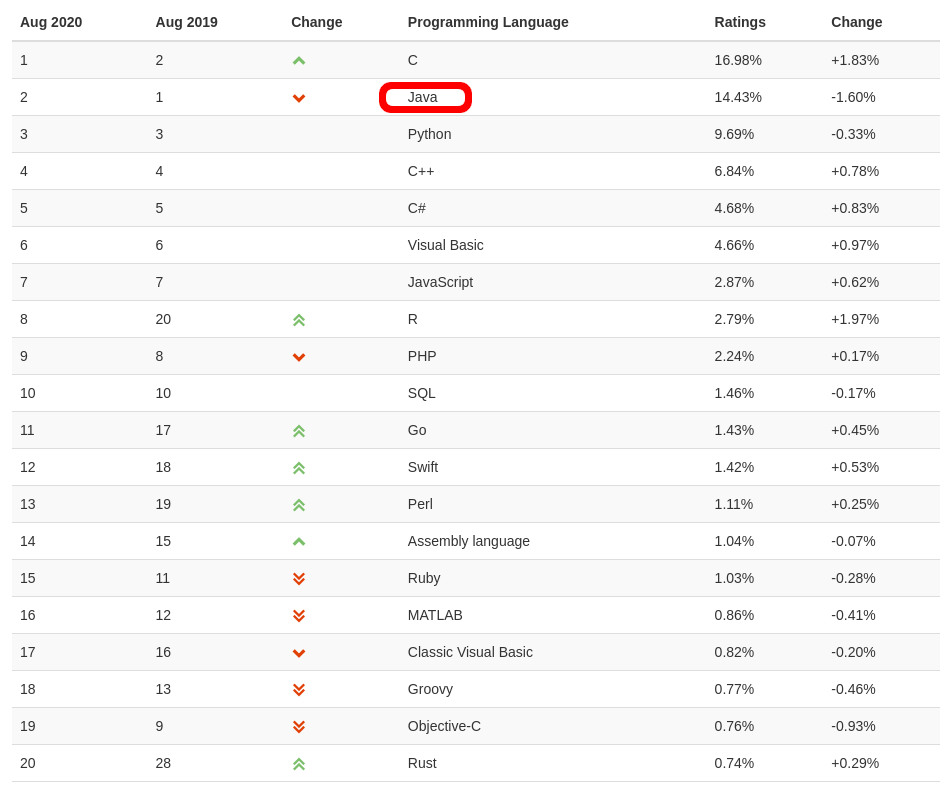
\includegraphics[height=8.3cm]{images01/2020_08_TIOBEIndex.png}
    \end{center}
    \caption{TIOBE Index as of 08/2020}
    \label{fig:TIOBEIdx}
  \end{figure}
\end{frame}

%%%%%%%%%%%%%%%%%%%%%%%%%%%%%%%%%%%%%%%%%%%%%%%%%%%%%%%%%%%%%%%%%%%%%%
\begin{frame}{Java:What \& Why}
  \hspace{3cm}
  \begin{itemize}
    \item \href{https://www.jmdoudoux.fr/java/dej/chap-presentation.htm}{In~2011}:
    \begin{itemize}
      \item \textbf{97\% of machines} have a JVM in enterprises
      \medskip
      \item \textbf{9~millions+ Java developers} in the world
      \medskip
      \item \textbf{3~billions+ mobile devices} run Java (Android\ldots{})
      \medskip
    \end{itemize}
  \end{itemize}
  \medskip
  \begin{itemize}
    \item \href{https://www.codeplatoon.org/best-paying-most-in-demand-programming-languages-2020/}{In~2020}:
    \begin{itemize}
      \item 3rd in \textbf{Job Postings}
      \item 3rd in \textbf{Average Salary}
    \end{itemize}
%
  \item \href{https://blogs.oracle.com/javamagazine/the-top-25-greatest-java-apps-ever-written}{Many Known Apps}: Minecraft, Wikipedia (search), NASA (Maestro Mars Rover), NSA (\href{https://www.wired.com/story/nsa-ghidra-open-source-tool/}{Ghidra}!) % WikiLeaks
%
  \end{itemize}

\bigskip
  \begin{center}
    
\includegraphics[height=8.3cm]{images01/earth1.png}
  \end{center}

\end{frame}

%%%%%%%%%%%%%%%%%%%%%%%%%%%%%%%%%%%%%%%%%%%%%%%%%%%%%%%%%%%%%%%%%%%%%%
\begin{frame}{Don't get it wrong}
  \begin{center}
    Java IS \textbf{NOT} JavaScript \\[1.5em]
    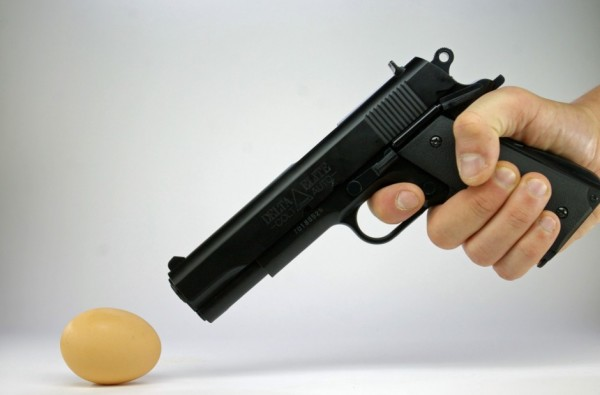
\includegraphics[width=.8\linewidth,height=.6\textheight]{./images01/killegg.jpg}
  \end{center}
\end{frame}

%%%%%%%%%%%%%%%%%%%%%%%%%%%%%%%%%%%%%%%%%%%%%%%%%%%%%%%%%%%%%%%%%%%%%%
\begin{frame}{Characteristics}
  \begin{itemize}
    \item Both \textbf{Compiled} (to bytecode) \& \textbf{Interpreted} (on the JVM)
    \vspace{.5em}
    \item \textbf{Hardware independent} ($\Rightarrow$ truly portable)\\
     \raisebox{-.5\height}{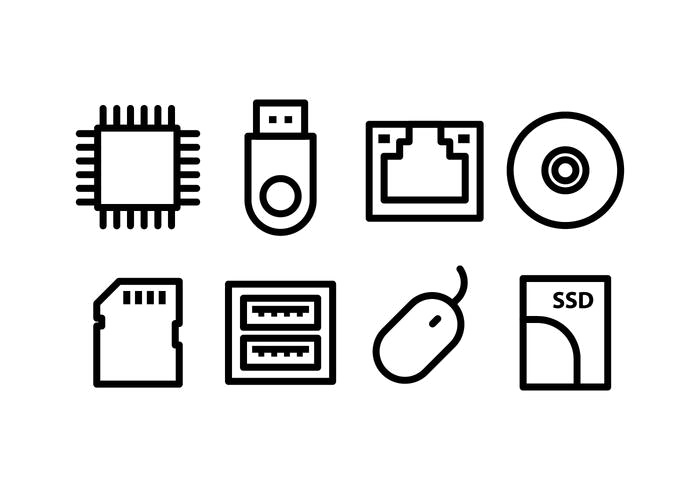
\includegraphics[height=4em]{images01/computer-hardware.png}}
     \raisebox{-.5\height}{
\includegraphics[height=2em]{images01/oses.png}}
    \vspace{.5em}
    \item \textbf{Strongly Typed}
    \raisebox{-.5\height}{
\includegraphics[height=4em]{images01/types.png}}
    \vspace{.5em}
    \item \textbf{Object Oriented}
    \vspace{.5em}
    \item Java manages the memory
    \hspace{3.3cm}\raisebox{-.6\height}{
\includegraphics[height=4em]{images01/GarbageCollector.png}}\\[-1em]
    (\textbf{NO} explicit \textbf{pointers} \texttt{\textbackslash{}o/}, Garbage Collector)
  \end{itemize}
\end{frame}

%%%%%%%%%%%%%%%%%%%%%%%%%%%%%%%%%%%%%%%%%%%%%%%%%%%%%%%%%%%%%%%%%%%%%%
\begin{frame}{Distributions}

  There are several \textbf{distributions} of Java
  \bigskip
  \begin{itemize}
    \item[\textbullet] \href{https://www.oracle.com/java/technologies/javase-downloads.html}{Sun/Oracle} vs.
          \href{https://adoptopenjdk.net/installation.html}{OpenJDK} vs.
          \href{https://www.eclipse.org/openj9/}{Eclipse} vs. %% https://www.eclipse.org/eclipse/news/4.10/jdt.php
          \href{https://en.wikipedia.org/wiki/GNU_Compiler_for_Java}{GNU}\ldots{}
    \medskip
    \item[\textbullet] \textcolor{blue}{\bf JRE}: Java Runtime Environment
    \begin{itemize}
      \item \textbf{Execution} environment only (JVM)
      \item $\Rightarrow$ for \textcolor{blue}{\bf end users}!
    \end{itemize}
%
    \item[\textcolor{red}{\textbullet}] \textcolor{red}{\bf JDK}: Java Development Kit
    \begin{itemize}
      \item Tools \& APIs to \textbf{develop} in Java
      \item $\Rightarrow$ for \textcolor{red}{\bf devs}!
    \end{itemize}
%
    \item[\textbullet] \textcolor{DarkGreen}{\bf J2EE}: Java Enterprise Edition
    \begin{itemize}
      \item JDK + tools \& APIs for \textcolor{DarkGreen}{\bf web development}
    \end{itemize}
  \end{itemize}

  \bigskip
  \textbf{Note: Installing a JDK also installs a JRE!}

\end{frame}


%%%%%%%%%%%%%%%%%%%%%%%%%%%%%%%%%%%%%%%%%%%%%%%%%%%%%%%%%%%%%%%%%%%%%%
\begin{frame}{Versions}
%
  \begin{itemize}
    \item \textbf{Since~2017}: 1~new version every 6~months
    \begin{itemize}
      \item New Features vs. LTS system
      \item Today (2020): latest = Java~14
      \item Big changes in Java~8 (Collections, Stream, \textbf{Lambdas})
      \item Java is \textbf{backward compatible}
    \end{itemize}
    \medskip
    \item Check installed version (Command Prompt)\\
    \texttt{\$ java -version}\\
    \texttt{openjdk version "11.0.8" 2020-07-14}
  \end{itemize}

\end{frame}

%%%%%%%%%%%%%%%%%%%%%%%%%%%%%%%%%%%%%%%%%%%%%%%%%%%%%%%%%%%%%%%%%%%%%%
\begin{frame}{Specificities}

  The Java platform has some \textbf{specificities}:
  \medskip
  \begin{itemize}
    \item A \textbf{single} (public) class per \texttt{java} source file
    \medskip
    \item \textbf{Compiles} source code into bytecode (hardware independent)
    \medskip
    \item This \textbf{bytecode} is executed (\textbf{interpreted}) on the \textbf{JVM}\footnote{\textbf{J}ava \textbf{V}irtual \textbf{M}achine}
    \medskip
    \item \textbf{No} header files, \textbf{no} linking
    \medskip
    \item \textbf{Packages} allow to organize code (\textbf{Classes})
    \medskip
    \item \texttt{jar} (\textbf{J}ava \textbf{AR}chive): format to distribute an ``executable''
    \medskip
    \item \textbf{CLASSPATH} indicates where to find classes
  \end{itemize}

\end{frame}

% %%%%%%%%%%%%%%%%%%%%%%%%%%%%%%%%%%%%%%%%%%%%%%%%%%%%%%%%%%%%%%%%%%%%%%
% \begin{frame}{Specificities}

%   \begin{center}
%     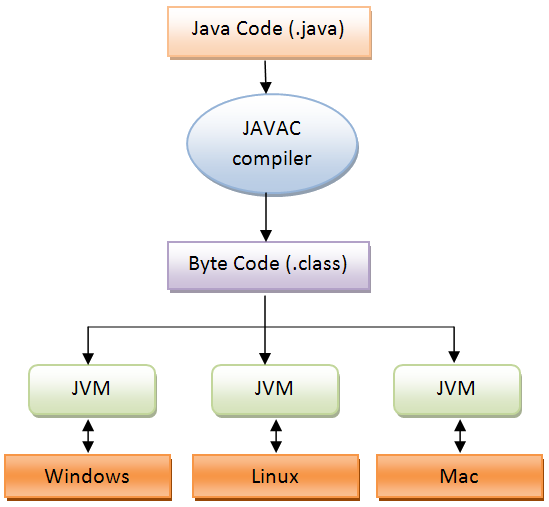
\includegraphics[height=.6\textheight]{./images01/jvm.png}
%   \end{center}

% \end{frame}

\section{Functioning}

\subsection{General Compilation Chain\footnote{Images from "Java Head First'' book.}}

%%%%%%%%%%%%%%%%%%%%%%%%%%%%%%%%%%%%%%%%%%%%%%%%%%%%%%%%%%%%%%%%%%%%%%
\begin{frame}{Compilation Chain -- User's View}

\centering{
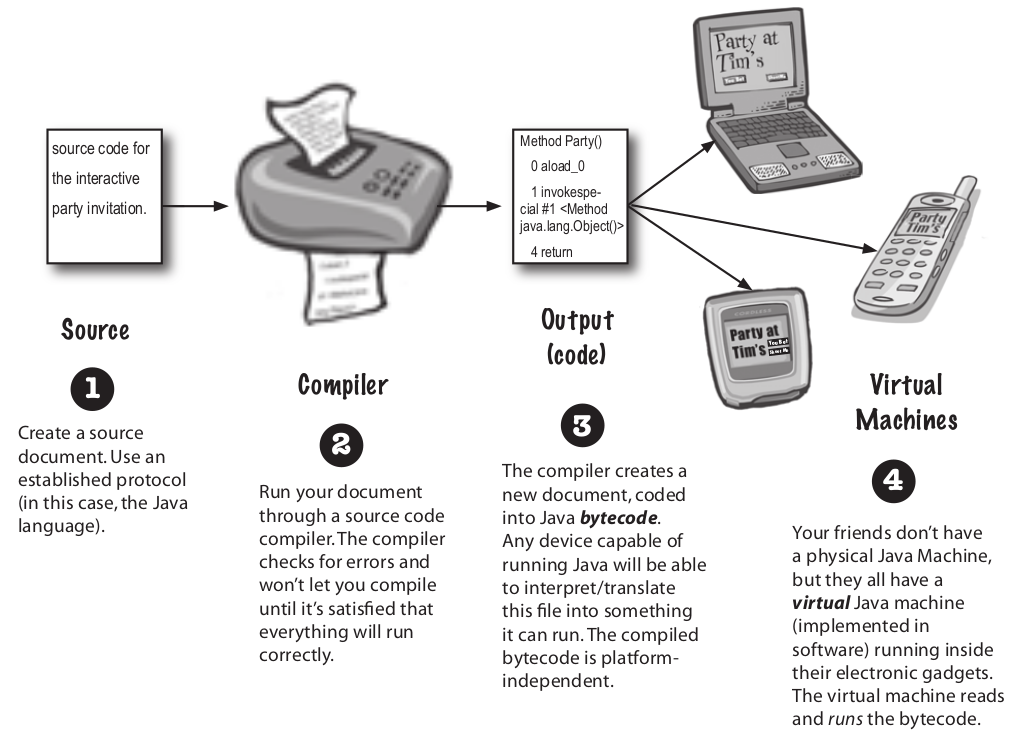
\includegraphics[height=0.85\textheight]{./images01/java_intro_compilationchain1.png}
}

\end{frame}

%%%%%%%%%%%%%%%%%%%%%%%%%%%%%%%%%%%%%%%%%%%%%%%%%%%%%%%%%%%%%%%%%%%%%%
\begin{frame}{Compilation Chain -- Developer's View}

\centering{
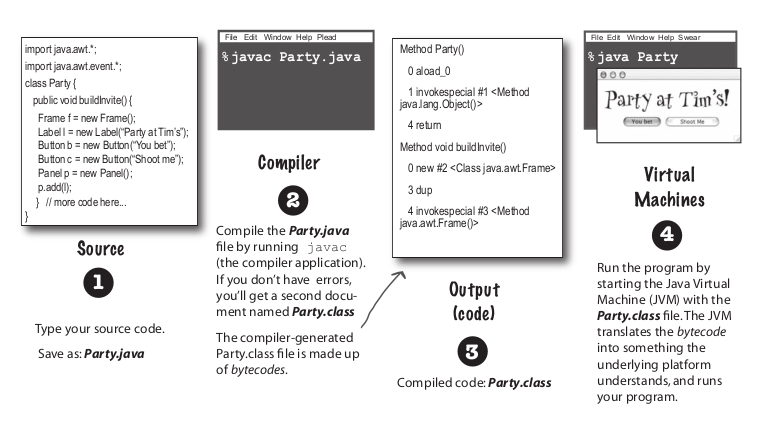
\includegraphics[height=0.7\textheight]{./images01/java_intro_compilationchain2.png}
}

\end{frame}

%%%%%%%%%%%%%%%%%%%%%%%%%%%%%%%%%%%%%%%%%%%%%%%%%%%%%%%%%%%%%%%%%%%%%%
\begin{frame}{Source code \& bytecode}
  \begin{itemize}
    \item Source code in \texttt{MyClass.java} file\footnote{One single (public) class per file}
    \medskip
    \item File name = (public) class name
    \medskip
    \item Compile with (\textbf{java c}ompiler): \\
    \texttt{javac <file>.java}
    \medskip
    \item Results in \texttt{.class} file (bytecode)
    \medskip
    \item Execute with (JVM):\\
    \texttt{javac <file>}\footnote{NOTE: there is no extension here!}
  \end{itemize}
\end{frame}

%%%%%%%%%%%%%%%%%%%%%%%%%%%%%%%%%%%%%%%%%%%%%%%%%%%%%%%%%%%%%%%%%%%%%%
\begin{frame}{Source File (class $\approx$ C struct + methods)}

\centering{
  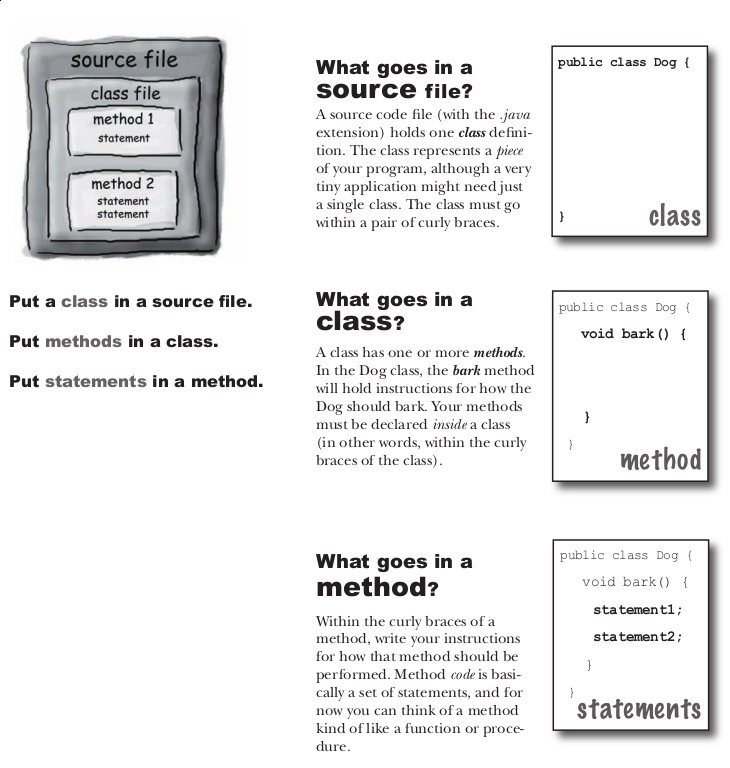
\includegraphics[height=0.8\textheight]{./images01/java_intro_sourcefile.png}
}

\end{frame}

%%%%%%%%%%%%%%%%%%%%%%%%%%%%%%%%%%%%%%%%%%%%%%%%%%%%%%%%%%%%%%%%%%%%%%
\begin{frame}{Compilation Chain -- First Run}

\centering{
  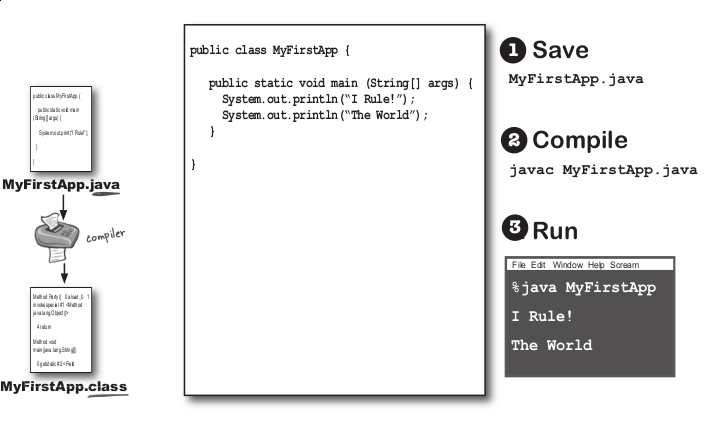
\includegraphics[height=0.8\textheight]{./images01/java_intro_compilationchain3.png}
}

\end{frame}

%%%%%%%%%%%%%%%%%%%%%%%%%%%%%%%%%%%%%%%%%%%%%%%%%%%%%%%%%%%%%%%%%%%%%%
\begin{frame}{My First Class}

\centering{
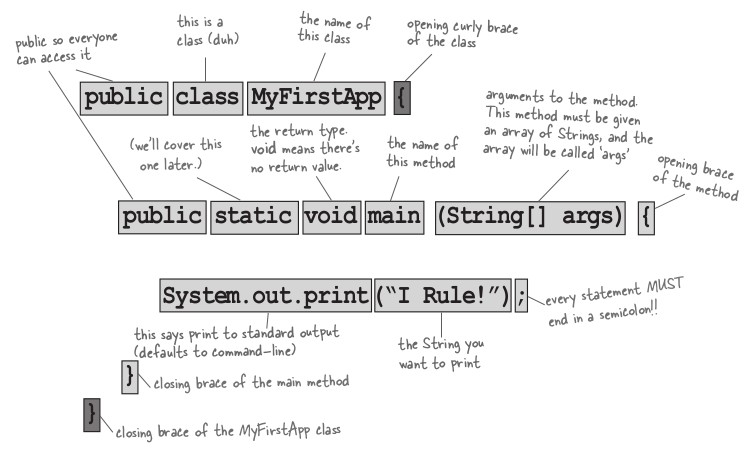
\includegraphics[height=0.8\textheight]{./images01/java_intro_class1.png}
}

\end{frame}

% %%%%%%%%%%%%%%%%%%%%%%%%%%%%%%%%%%%%%%%%%%%%%%%%%%%%%%%%%%%%%%%%%%%%%%
% \begin{frame}{Class File Content}

% \centering{
% 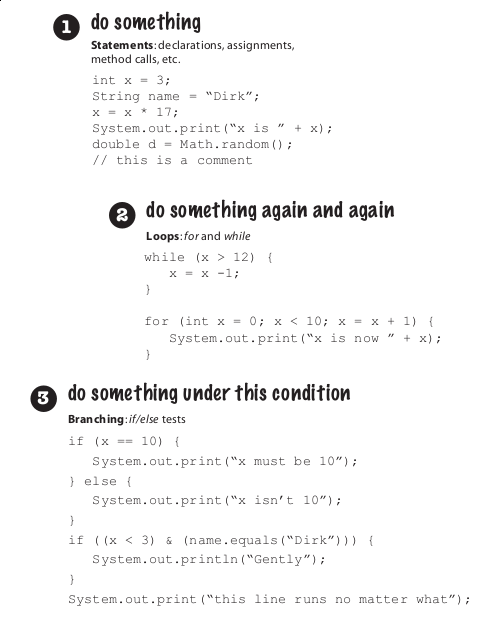
\includegraphics[height=0.8\textheight]{./images01/java_intro_class2.png}
% }

% \end{frame}

\subsection{Keywords}
   \begin{frame}{Outline}
       \tableofcontents[currentsubsection]
   \end{frame}

%%%%%%%%%%%%%%%%%%%%%%%%%%%%%%%%%%%%%%%%%%%%%%%%%%%%%%%%%%%%%%%%%%%%%%
\begin{frame}{Java Keywords}

%\vspace{-.2em}
  { \footnotesize
  \begin{itemize}

    \item \textbf{Comments}: \texttt{/* comnent */}, \texttt{/** Java Doc */}, \texttt{// single line} \\

    \item (Basic) \textbf{Types}: \\
    \texttt{\color{red} void}, \texttt{boolean}, \texttt{char}, \texttt{byte},
    \texttt{short}, \texttt{int}, \texttt{float}, \texttt{long},
    \texttt{double}, \texttt{\color{red} []}\\
    \texttt{\color{red} String}, \texttt{\color{red} List}, \texttt{\color{red} Set}, \texttt{\color{red} Map}\ldots{}

    \item \textbf{Control Structures}: \\
    \texttt{for}, \texttt{while}/\texttt{do},
    \texttt{break}/\texttt{continue}\\
    \texttt{if}/\texttt{else}, \texttt{switch}/\texttt{case}

    \item \textbf{Methods}: \texttt{return}, \texttt{super}

    \item \textbf{Packages}: \texttt{package}, \texttt{import}

    \item \textbf{Objects}:\\
    \texttt{interface}/\texttt{class}, \texttt{abstract},
    \texttt{implements}, \texttt{extends}\\
    \texttt{new}, \texttt{this}\\
    \texttt{static}, \texttt{final}

    \item \textbf{Visibility}: \texttt{private}, \texttt{public}, \texttt{protected}

    \item \textbf{Exceptions}:\\
    \texttt{throw}/\texttt{throws}, \texttt{try}/\texttt{catch}/\texttt{finally}

  \end{itemize}
}

\end{frame}

\subsection{Naming Conventions}
   \begin{frame}{Outline}
       \tableofcontents[currentsubsection]
   \end{frame}

%%%%%%%%%%%%%%%%%%%%%%%%%%%%%%%%%%%%%%%%%%%%%%%%%%%%%%%%%%%%%%%%%%%%%%
\begin{frame}[fragile]{Naming Conventions}

{\small
  \begin{itemize}
%
    \item \textbf{Packages}: lowercase + dots \\
\begin{verbatim}
    com.sun.eng
\end{verbatim} % cannot be indented ? :{
    %
    \item \textbf{Classes / Interfaces}: (upper) CamelCase\\
\begin{verbatim}
    class ImageSprite;
    interface RasterDelegate;
\end{verbatim}
%
    \item \textbf{Methods}: dromedaryCase == (lower) camelCase \\
\begin{verbatim}
    run();
    runFast();
\end{verbatim}
%
    \item \textbf{Variables / Attributes}: dromedaryCase \\
\begin{verbatim}
    int             i;
    char            c;
    float           myWidth;
\end{verbatim}
%
    \item \textbf{Constants}: ALL CAPS + snake\_case \\
\begin{verbatim}
    static final int MIN_WIDTH = 4;
\end{verbatim}
%
\end{itemize}
}

\end{frame}

\subsection{Pointers/References}
   \begin{frame}{Outline}
       \tableofcontents[currentsubsection]
   \end{frame}

%%%%%%%%%%%%%%%%%%%%%%%%%%%%%%%%%%%%%%%%%%%%%%%%%%%%%%%%%%%%%%%%%%%%%%
\begin{frame}[fragile]{Pointers and parameters}

\begin{minipage}[l]{.45\textwidth}
  \begin{lstlisting}[escapechar=\%,label=inCpp,caption=MyCode.cpp]
    Pair origin;
    Pair *p, *q, *r;
    origin.x = 0;
    p = new Pair;
    p -> y = 5;
    q = p;
    r =  & origin;
   \end{lstlisting}
 \end{minipage}
 \begin{minipage}[l]{.45\textwidth}
   \begin{lstlisting}[escapechar=\%,label=inJava,caption=MyCode.java]
     Pair origin = new Pair();
     Pair p, q, r;
     origin.x = 0;
     p = new Pair();
     p.y = 5;
     q = p;
     // not possible
   \end{lstlisting}
 \end{minipage}

\bigskip
\bigskip

\danger{}~Objects in Collections \textbf{can be modified}!!! \\
(behind the hood, the Collection contains references)!!!

\end{frame}


%%%%%%%%%%%%%%%%%%%%%%%%%%%%%%%%%%%%%%%%%%%%%%%%%%%%%%%%%%%%%%%%%%%%%%
\begin{frame}{No \texttt{delete}?}
  \vspace{.2em}
  \begin{itemize}
    \item<1-> The \texttt{new} keyword creates instances
    \item<1-> There is \textbf{no} \texttt{delete} in Java!!!
  \end{itemize}
  \bigskip
  \onslide<2->{
    \begin{minipage}[c]{.90\linewidth}
      \begin{itemize}
        \item \textbf{Java manages the memory itself}
        \item The «~\textbf{Garbage Collector}~» does the job
        \textit{It's a module of the JVM that removes Objects from memory
          when they are not used (referenced) anymore}
        \pause
      \end{itemize}
    \end{minipage}
    \begin{minipage}[c]{.05\linewidth}
      
\includegraphics[height=2em]{images01/GarbageCollector.png}
    \end{minipage}
  }
\onslide<3->{
  \begin{itemize}
    \item \textbf{Pros?} \textbf{Cons?}
  \end{itemize}
}
\onslide<4->{
  \centering{
    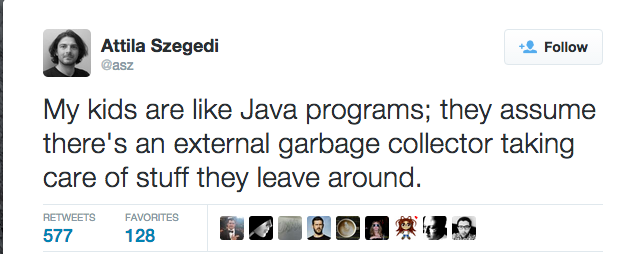
\includegraphics[height=0.4\textheight]{./images01/garbage.png}
  }
}
\end{frame}


\subsection{Packages}
   \begin{frame}{Outline}
       \tableofcontents[currentsubsection]
   \end{frame}

% %%%%%%%%%%%%%%%%%%%%%%%%%%%%%%%%%%%%%%%%%%%%%%%%%%%%%%%%%%%%%%%%%%%%%%
% \begin{frame}{On Bytecode and Just-In-Time compilation}

% Pros:
% \begin{itemize}
%     \item Online methods
%     \item Eliminate locks
%     \item Join adjacent synchronized blocks
%     \item Eliminate Dead Code
%     \item etc.
% \end{itemize}

% \pause

% Cons:
% \begin{itemize}
%     \item Increase memory heap,
%     \item Loading time,
%     \item Even more code modification than traditional compiler.
% \end{itemize}

% \end{frame}

%%%%%%%%%%%%%%%%%%%%%%%%%%%%%%%%%%%%%%%%%%%%%%%%%%%%%%%%%%%%%%%%%%%%%%
\begin{frame}[fragile]{Example}
\begin{lstlisting}[escapechar=\%,label=hellojava,caption=MyClass.java]
public class MyClass {
  public static void main(String[] args) {
    System.out.println("Hello World!");
  }
}
\end{lstlisting}

\bigskip

\begin{itemize}
    \item To compile (creates bytecode into \texttt{hello.class}): \\
    \texttt{javac MyClass.java}
    \item To excute (no extension! it the class name!): \\
    \texttt{java MyClass}
    \item Result: \\
    \texttt{$\|$ Hello World!}
\end{itemize}

\end{frame}

%%%%%%%%%%%%%%%%%%%%%%%%%%%%%%%%%%%%%%%%%%%%%%%%%%%%%%%%%%%%%%%%%%%%%%
\begin{frame}[fragile]{Packages}

\begin{lstlisting}[escapechar=\%,label=hellopackage,caption=HelloWorld.java]
package fr.tse.java;      // Declare Package (name == dir. where stored!!)
import java.util.List; // Refers to another class in another Pacakge

public class HelloWorld {
  public static void main(String[] args) {
    List myList = ...;
  }
}
\end{lstlisting}

{\scriptsize
\begin{itemize}
    \item Source code is organized in «~packages~»
    \item Strings separated by points (\texttt{.})
    \item Similar to file path: \textbf{it is indeed!} \\
    File: \texttt{fr/tse/java/HelloWorld.java}
    \medskip
    \item To compile: \\
    \texttt{javac fr/tse/java/MyClass.java}
    \item To excute (FQN): \\
    \texttt{java fr.tse.java.MyClass}
\end{itemize}
}

\end{frame}

%%%%%%%%%%%%%%%%%%%%%%%%%%%%%%%%%%%%%%%%%%%%%%%%%%%%%%%%%%%%%%%%%%%%%%
\begin{frame}{Packages included in Java platform}

\begin{itemize}
  \item \texttt{java.lang}: Basic classes \hfill \textit{imported automatically}\\
  \texttt{String}, \texttt{Character}, \texttt{Integer}\ldots{}\\
%
  \medskip
  \item \texttt{java.io}: Input/Output\\
  \texttt{File}\ldots{}
%
  \medskip
  \item \texttt{java.util}: useful structures \& methods\\
  \texttt{Collections}, \texttt{List}, \texttt{Set}, \texttt{Random}\ldots{}
%
  \medskip
  \item \texttt{java.math}: math operations
  \texttt{cos()}, \texttt{sin()}\ldots{}
%
  \medskip
  \item \ldots{}
%
  \bigskip
  \item Extensive list in the official doc:\\
  \url{http://docs.oracle.com/javase/8/docs/api/}
\end{itemize}

\end{frame}


%%%%%%%%%%%%%%%%%%%%%%%%%%%%%%%%%%%%%%%%%%%%%%%%%%%%%%%%%%%%%%%%%%%%%%
\begin{frame}[fragile]{Example of importing \texttt{java.util.ArrayList}}

\begin{lstlisting}[escapechar=\%,label=myarraylistpackage,caption=MyArrayList.java]
package fr.tse.java;

import java.util.ArrayList;

public class MyArrayList {
  public static void main(String[] args) {
    System.out.println("Bonjour");
    ArrayList<String> v = new ArrayList<String>();
    // Remember: Java is strongly typed, hence <...>!
  }
}
\end{lstlisting}

  \bigskip
\begin{itemize}
  \item Description of Java's ArrayList class:\\
  \url{http://docs.oracle.com/javase/8/docs/api/java/util/ArrayList.html}
\end{itemize}

\end{frame}


\subsection{JAR files}
   \begin{frame}{Outline}
       \tableofcontents[currentsubsection]
   \end{frame}

%%%%%%%%%%%%%%%%%%%%%%%%%%%%%%%%%%%%%%%%%%%%%%%%%%%%%%%%%%%%%%%%%%%%%%
\begin{frame}{Java ARchive (JAR files)}
\begin{itemize}
    \item Assemble all the \texttt{.class} files into an executable\footnote{A Java ARchive (JAR) file, with extension \texttt{.jar}}\\
    \texttt{jar -cf MyClass.jar ./fr}
    \pause
    \medskip
    \item Execute this \texttt{jar} file\\
    \texttt{java -jar MyClass.jar}
    \pause
    \medskip
    \item Requires the name of the main Class (entry point: \texttt{main()}):
    \begin{itemize}
      \item Config file: \texttt{./META-INF/MANIFEST.MF}:\\
      \texttt{Main-Class: fr.tse.java.MyClass}
      \item Add this file to the \texttt{jar}:\\
      \texttt{jar -cmvf MyClass.jar ./fr}
    \end{itemize}
\end{itemize}
\end{frame}


\subsection{Classpath}
   \begin{frame}{Outline}
       \tableofcontents[currentsubsection]
   \end{frame}

%%%%%%%%%%%%%%%%%%%%%%%%%%%%%%%%%%%%%%%%%%%%%%%%%%%%%%%%%%%%%%%%%%%%%%
\begin{frame}{Classpath}
  \begin{itemize}
    \item Context:
    \begin{itemize}
      \item My code is in a \texttt{jar} file
      \item It \texttt{imports} library classes from other \texttt{jar} files
    \end{itemize}
    \medskip
    \item Problem: How do I tell the JVM where to look for \texttt{import}ed classes?
    \pause
    \bigskip
    \item Solution: The \textbf{CLASSPATH}, is a list of all the pathes where to find these librairies (both Java's and our own's)
  \end{itemize}
\end{frame}


%%%%%%%%%%%%%%%%%%%%%%%%%%%%%%%%%%%%%%%%%%%%%%%%%%%%%%%%%%%%%%%%%%%%%%
\begin{frame}{Classpath}
  \begin{itemize}
    \item \textbf{CLASSPATH} = list of pathes to external code
\medskip
    \item It is generally stored in an Environment Variable
    \item Each element can be:
    \begin{itemize}
      \item A directory (with \texttt{.class} in its sub-directories)
      \item A \texttt{.jar}
      \item A \texttt{.zip} file (mostly used internally by JVM)
    \end{itemize}
    \item Separator: \texttt{``:''} (Unices: Linux/MacOS) or \texttt{``;''} (Windows)
\end{itemize}
\bigskip
Example of a CLASSPATH:\\
{\footnotesize \texttt{.:/home/prog/lib/:/usr/lib/java/log4j-1.2.11.jar:../lib-ext/junit.jar}}
\end{frame}

%%%%%%%%%%%%%%%%%%%%%%%%%%%%%%%%%%%%%%%%%%%%%%%%%%%%%%%%%%%%%%%%%%%%%%
\begin{frame}{Classpath -- Example}

{\footnotesize
  \texttt{
    \textcolor{red}{.}:\textcolor{green}{/home/prog/lib/}:\textcolor{blue}{/usr/lib/java/log4j-1.2.11.jar}:\textcolor{brown}{../lib-ext/junit.jar}
  }
}
is composed of:
\begin{itemize}
    \item All \texttt{.class} in current directory (\texttt{\textcolor{red}{.}} \& subdirs)
    \item All \texttt{.class} in \texttt{\textcolor{green}{/home/prog/lib/}} (\& subdirs)
    \item Classes from archive \texttt{\textcolor{blue}{log4j-1.2.11.jar}} found in\\
    \textit{absolute} path \texttt{\textcolor{blue}{/usr/lib/java/}}
    \item Classes form archive \texttt{\textcolor{brown}{junit.jar}} found in\\
    \textit{relative} path \texttt{\textcolor{brown}{../lib-ext/}}
\end{itemize}
\end{frame}


%%%%%%%%%%%%%%%%%%%%%%%%%%%%%%%%%%%%%%%%%%%%%%%%%%%%%%%%%%%%%%%%%%%%%%
\begin{frame}{How to provide the \textbf{classpath} compile/run-time?}
  \begin{itemize}
    \item Option \texttt{-classpath} du compilateur
    \begin{itemize}
      \item \texttt{javac -classpath ./:/home/prog/lib/  MyClass.java}
    \end{itemize}
    \bigskip
    \item Option \texttt{-cp} of the JVM
    \begin{itemize}
      \item \texttt{java -cp ./:/home/prog/lib/  MyClass}
      \item \texttt{java -cp ./:/home/prog/lib/  fr.tse.java.MyClass}
    \end{itemize}
  \end{itemize}
\end{frame}


\section{Your turn}

\subsection{Java -- Manually}

%%%%%%%%%%%%%%%%%%%%%%%%%%%%%%%%%%%%%%%%%%%%%%%%%%%%%%%%%%%%%%%%%%%%%%
\begin{frame}{Sump Up -- Running Java Manually}
Let's do a live coding demo with Text Editor+Command Line!!!
\begin{itemize}
  \item Open a text editor
  \item Create a \texttt{HelloWorld.java} file + Type a \texttt{HelloWorld} class
  \item Compile with \texttt{javac}
  \item Run with \texttt{java}
  \medskip
  \item Create a \texttt{fr/tse/java} dir hierarchy
  \item Move the class in this directory
  \item Try to run the class $\Rightarrow$ does not work
  \item Add the \texttt{package} directive $\Rightarrow$ it works!!
  \medskip
  \item Create a \texttt{jar} file
  \item Try to execute it with \texttt{java -jar} $\Rightarrow$ does not work
  \item Correct it to add \texttt{./META-INF/MANIFEST.MF} file
\end{itemize}
\end{frame}

\subsection{Java -- with Eclipse}
%%%%%%%%%%%%%%%%%%%%%%%%%%%%%%%%%%%%%%%%%%%%%%%%%%%%%%%%%%%%%%%%%%%%%%
\begin{frame}{Sump Up -- Eclipse}
Let's do a 2$^{\text{nd}}$ live coding demo, with Eclipse IDE!!!
\begin{itemize}
  \item Start Eclipse
  \item Select workspace (\& accept forever?)
  \item Create a \textbf{Java/Maven Project}
  \item Observe the Project herarchy is automatically created
  \medskip
  \item Create a Package $\Rightarrow$ the dirs are created automatically
  \item Create a Class $\Rightarrow$ file/class names correspond!
  \medskip
  \item Use autocompletion to create \texttt{main}
  \item Use autocompletion to enter \texttt{sysout}
  \medskip
  \item Generate a \texttt{.jar} file
\end{itemize}
\end{frame}


\section{Resources}

%%%%%%%%%%%%%%%%%%%%%%%%%%%%%%%%%%%%%%%%%%%%%%%%%%%%%%%%%%%%%%%%%%%%%%
\begin{frame}{Resources}

%\vspace{-.5em}

% TODO: Dépasse => splitter en 2 ?

\hspace*{-1cm}{\tiny
\begin{itemize}

  \item \textbf{Official Docs}\\
  \url{https://docs.oracle.com/javase/tutorial/} \\
  \url{https://docs.oracle.com/javase/8/docs/api/}

  \item \textbf{Eclipse Key Bindings CheatSheet}\\
  \url{https://mootse.telecom-st-etienne.fr/pluginfile.php/9061/mod_resource/content/1/EclipseShortcutCheatSheet.pdf}

  \item \textbf{A few useful CheatSheets}\\
  \url{https://dzone.com/refcardz/getting-started-eclipse}\\
  \url{https://dzone.com/refcardz/core-java}\\
  \url{https://dzone.com/refcardz/getting-started-java-gui} \\
  \url{https://dzone.com/refcardz/apache-maven-2} \\
  \url{https://dzone.com/refcardz/getting-started-git} \\
  \url{https://www.jrebel.com/system/files/git-cheat-sheet.pdf}\\
  \url{https://www.jrebel.com/search/results?keys=cheat\%20sheet}

  \item \textbf{Tutorials sites}\\
  \url{https://www.baeldung.com/}\\
  \url{https://www.tutorialspoint.com/java/index.htm}\\

  \item \textbf{News sites}\\
  \url{https://dzone.com/}\\
  \url{https://jrebel.com/resources/}\\
  \url{https://www.infoq.com/}

  \item \textbf{Complete course}\\
  \url{http://jmdoudoux.developpez.com/cours/developpons/java/}

  \item \textbf{Glossary}\\
  \url{http://mindprod.com/jgloss/jcheat.html}\\
  \url{https://dzone.com/articles/java-glossary-and-the-core-concepts}

  \item \textbf{Quizzes}\\
  \url{https://www.w3schools.com/java/}

  \item \textbf{Books}: [\textbf{UK}] NoStarch, OReilly, Manning, Packt ; [\textbf{FR}] Eyrolles, Dunod

% Git: https://git-scm.com/book/en/v2

  \item \textbf{Programming cleanly}\\
  \url{https://www.worldcat.org/title/java-by-comparison-become-a-java-craftsman-in-70-examples/oclc/1035454599} \\
  \url{https://github.com/GMTSE/ProjetsJavaMaterial/blob/master/JavaByComparisonSumUp.md}

\end{itemize}
}

\end{frame}



\section{Summary}
%%%%%%%%%%%%%%%%%%%%%%%%%%%%%%%%%%%%%%%%%%%%%%%%%%%%%%%%%%%%%%%%%%%%%%
\begin{frame}{Sump Up}
  \begin{itemize}
    \item Java follows \textbf{OOP paradigm}
    \item Java is \textbf{widely used}
\medskip
    \item Code in \texttt{.java} files (filename = Class name)
    \item Code organized in \textbf{packages} (many provided in Java platform)
    \item Compile\\
    \texttt{javac MyClass.java}
    \item Execute\\
    \texttt{java MyClass}
\medskip
    \item We will learn \textbf{Java~8} features
    \item We will use \textbf{Eclipse} to write code
    \item We will use \textbf{Maven} to compile/manage deps
  \end{itemize}
\end{frame}

\end{document}